%\documentclass[titlepage, a4paper, 12pt, reqno, openany]{beamer}
%\documentclass[12pt]{beamer}
\documentclass[aspectratio=169]{beamer}
%%%%%%%%%%%%%%%%%%%%%%%%%%%%%%%%%%%%%%%%%%%%%%%%%%%%%%%%%%%%%%%%%%%%%%%%%%%%%
%%%%%%encoding%%%%%%
\usepackage[T1]{fontenc}
\usepackage[utf8]{inputenc}
\usepackage[portuguese]{babel}
%%%%%%Hyphenation rules%%%%%%
\usepackage{babelbib}
\usepackage{float}
\usepackage{amsfonts}
\usepackage{amsmath}
\usepackage{amssymb}
\usepackage{color,colortbl}
%\usepackage[usenames,dvipsnames,svgnames,table]{xcolor} %permite letras coloridas
\usepackage{verbatim}
%%%%%%%%%%%%%%%%%%%%%%%%%%%%%%BEAMER THEMES%%%%%%%%%%%%%%%%%%%%%%%%%%%%%%%%%%%%
\usetheme{Frankfurt}
%\usetheme{Boadilla}
%\usetheme{Warsaw}
%%%%%%%%%%%%%%%%%%%%%%%%%%%%%BEAMER PACKAGES%%%%%%%%%%%%%%%%%%%%%%%%%%%%%%%%%%%
%\usepackage{smartdiagram}
%%%%%%%%%%%%%%%%%%%%%%%%%%%%%%%%%%%%%%%%%%%%%%%%%%%%%%%%%%%%%%%%%%%%%%%%%%%%%%%
\usepackage{graphicx} %permite inserir figuras
\usepackage{multicol}
\usepackage{multirow}
\usepackage{makecell}
\usepackage{adjustbox}
\usepackage{setspace} %distancia entree linhas
%\usepackage{times}
%\usepackage{hyphenat}
%\usepackage{makeidx} %para criar índice remissivo
%\usepackage{array}
%\usepackage{supertabular}
%\usepackage{bm}
%\usepackage{booktabs}
%\usepackage{boxedminipage}
%\usepackage{caption}
%\usepackage{changepage}
%\usepackage{cite}
%\usepackage{easylist}
%\usepackage{esint}
%\usepackage{eucal}
%\usepackage{fancyhdr}
%\usepackage{hyperref} %index dentro de red boxes
%\usepackage{indentfirst}
%\usepackage{latexsym}
%\usepackage{listings}
%\usepackage{mathptmx}
%\usepackage{mathrsfs} %permite o uso de letras trabalhadas
%\usepackage{microtype}
%\usepackage[normalem]{ulem} %permite sublinhar palavras
%\usepackage{paralist}
%\usepackage{pifont}
%\usepackage{rotating}
%\usepackage{setspace}
%\usepackage{syntonly} %speedup work desabling pdf converse \syntaxonly
%\usepackage{subfiles}
%\usepackage{subcaption}
%\usepackage{textcomp}
%\usepackage{theorem}
%\usepackage{ulem}
%\usepackage{url}
%\usepackage{wrapfig}
%%%%%recent%%%%%
%\usepackage{cancel}
%\usepackage[fleqn]{mathtools}
%\usepackage{pdfpages}
%\usepackage{pdflscape}
%\usepackage{todonotes}
%\usepackage{siunitx}
%%%%%%%%%%%%%%%%%%%%%%%%%%%%%%%%%%%%%%%%%%%%%%%%%%%%%%%%%%%%%%%%%%%%%%%%%%%%%%%%%%%
%\renewcommand\thesection{\arabic{section}}
%\renewcommand\thesubsection{\thesection.\arabic{subsection}}
%%%%%%%%%%%%%%%%%%%%%%%%%%%%%%%%%%%%%%%%%%%%%%%%%%%%%%%%%%%%%%%%%%%%%%%%%%%%%%%%%%%%
\begin{comment}
\usepackage{enumitem}
\setlistdepth{12}
\newlist{enumitem}{enumerate}{12}
\setlist[enumitem,1]{label=\roman*)}
\setlist[enumitem,2]{label=\alph*)}
\setlist[enumitem,3]{label=\arabic*)}
\setlist[enumitem,4]{label=(\roman*)}
\setlist[enumitem,5]{label=(\alph*)}
\setlist[enumitem,6]{label=(\arabic*)}
\setlist[enumitem,7]{label=\roman*)}
\setlist[enumitem,8]{label=\alph*)}
\setlist[enumitem,9]{label=\arabic*)}
\setlist[enumitem,10]{label=(\roman*)}
\setlist[enumitem,11]{label=(\alph*)}
\setlist[enumitem,12]{label=(\arabic*)}
\end{comment}

%%%%%%%%%%%%%%%%%%%%%%%%%%%%%%%%%%%%%%%%%%%%%%%%%%%%%%%%%%%%%%%%%%%%%%%%%%%%%%%%%%%%
\begin{comment}
\usepackage{enumerate}
\renewcommand{\labelitemi}{$\bullet$}
\renewcommand{\labelitemii}{$\cdot$}
\renewcommand{\labelitemiii}{$\diamond$}
\renewcommand{\labelitemiv}{$\ast$}
\end{comment}

%%%%%%%%%%%%%%%%%%%%%%%%%%%%%%%%%%%%%%%%%%%%%%%%%%%%%%%%%%%%%%%%%%%%%%%%%%%%%%%%%%%%

\usepackage{tikz}
\begin{comment}
\usepackage{circuitikz}
\usetikzlibrary{matrix,shapes.geometric,arrows,trees,positioning,calc}
\tikzstyle{RECTANGLE_2} = [rectangle, draw, text width=5em, text centered, rounded corners, minimum height=4em]
\tikzstyle{RECTANGLE_3} = [rectangle, rounded corners, minimum width=3cm, minimum height=1cm,text centered, draw=black, fill=red!80]
\tikzstyle{RECTANGLE_4} = [rectangle, draw, fill=blue!20, text width=3cm, text centered, minimum height=4em]
\tikzstyle{RECTANGLE_5} = [rectangle, minimum width=3cm, minimum height=1cm, text centered, text width=3cm]
\tikzstyle{RECTANGLE_6} = [rectangle, draw, fill=blue!20, text width=5em, text centered, rounded corners, minimum height=4em]
\tikzstyle{RECTANGLE_7} = [rectangle, draw, fill=blue!20, text width=5em, text centered, rounded corners, minimum height=4em]
\tikzstyle{RECTANGLE_8} = [rectangle, draw, align=left, fill=blue!20]
\tikzstyle{RECTANGLE_1} = [rectangle, rounded corners, minimum width=1cm, minimum height=1cm,text centered, draw=black, fill=green!%30]
\tikzstyle{DIAMOND_1} = [diamond, draw, fill=blue!20, text width=4.5em, text badly centered, node distance=4cm, inner sep=0pt]
\tikzstyle{DIAMOND_2} = [diamond, minimum width=3cm, minimum height=1cm, text centered, draw=black, fill=green!30]
\tikzstyle{DIAMOND_3} = [diamond, draw, text width=4.5em, text badly centered, node distance=3cm, inner sep=0pt]
\tikzstyle{DIAMOND_4} = [diamond, draw, fill=blue!20, text width=4.5em, text badly centered, node distance=3cm, inner sep=0pt]
\tikzstyle{DIAMOND_5} = [diamond, draw, fill=blue!20, text width=4.5em, text badly centered, node distance=3cm, inner sep=0pt]
\tikzstyle{DIAMOND_6} = [diamond, draw, fill=blue!20, text width=4.5em, text badly centered, node distance=4cm, inner sep=0pt]
\tikzstyle{DIAMOND_7} = [diamond, draw, align=left, fill=blue!20]
\tikzstyle{ELLIPSE_1} = [draw, ellipse,fill=red!20, node distance=3cm, minimum height=2em]
\tikzstyle{ELLIPSE_2} = [draw, ellipse,fill=red!20, node distance=3cm, minimum height=2em]
\tikzstyle{ELLIPSE} = [draw, ellipse,fill=red!20, node distance=3cm, minimum height=2em]
\tikzstyle{TRAPEZIUM_1} = [trapezium,trapezium left angle=70,trapezium right angle=-70,minimum height=0.6cm, draw, fill=blue!20, text width=4.5em, text badly centered, node distance=3cm, inner sep=0pt]
\tikzstyle{TRAPEZIUM_2} = [trapezium, trapezium left angle=70, trapezium right angle=110, minimum width=3cm, minimum height=1cm, text centered, draw=black, fill=blue!30]
\tikzstyle{TRAPEZIUM_3} = [trapezium,trapezium left angle=70,trapezium right angle=-70,minimum height=0.6cm, draw, fill=blue!20, text width=4.5em, text badly centered, node distance=3cm, inner sep=0pt]
\tikzstyle{ARROW} = [thick,->,>=stealth]
\tikzstyle{LINE} = [draw, -latex']
\tikzstyle{MYLINE} = [draw, ->,  thick, shorten <=4pt, shorten >=4pt]
\tikzstyle{TEXT_1}=[draw,text centered,minimum size=6em,text width=5.25cm,text height=0.34cm]
\tikzstyle{TEXT_2}=[draw,text centered,minimum size=2em,text width=2.75cm,text height=0.34cm]
\tikzstyle{TEXT_3}=[draw,minimum size=2.5em,text centered,text width=3.5cm]
\tikzstyle{TEXT_4}=[draw,minimum size=3em,text centered,text width=6.cm]
\tikzstyle{CIRCLE_1}=[draw,shape=circle,inner sep=2pt,text centered, node distance=3.5cm]
\tikzstyle{CIRCLE_2}=[draw,shape=circle,inner sep=4pt,text centered, node distance=3.cm]
\end{comment}

%%%%%%%%%%%%%%%%%%%%%%%%%%%%%%%%%%%%%%%%%%%%%%%%%%%%%%%%%%%%%%%%%%%%%%%%%%%%%%%%%%%%
%%%%%%%%%%%%%%%%%%%%%%%%%%%%%%%%%%%%%%%%%%%%%%%%%%%%%%%%%%%%%%%%%%%%%%%%%%%%%%%%%%%%
\makeindex
\bibliographystyle{babplain}
\begin{document}
\renewcommand\thesection{\arabic{section}}
\renewcommand\thesubsection{\thesection.\arabic{subsection}}
\renewcommand\thesubsubsection{\thesection.\thesubsection.\arabic{subsubsection}}

\begin{frame}
\frametitle{Plano de desenvolvimento pessoal de competências}
%\begin{figure}[ht]
%\begin{center}
%
\includegraphics[scale=0.2]{"./image/ROQ/Roq_LOGO.jpg"}
%\today{\date}
%\end{center}
%\end{figure}\par
\vfill
\hfill {\tiny Sérgio Santos}
\end{frame}
%\maketitle
%%%%%%%%%%%%%%%%%%%%%%%%%%%%%%%%%%%%%%%%%%%%%%%%%%%%%%%%%%%%%%%%%%%%%%%%%%%%%%%%%%%%%%%%%%%%%%%%%%%%%%%%%%%%%%%
%\begin{frame}{Nome da Organização}
%\tableofcontents
%\end{frame}
%%%%%%%%%%%%%%%%%%%%%%%%%%%%%%%%%%%%%%%%%%%%%%%%%%%%%%%%%%%%%%%%%%%%%%%%%%%%%%%%%%%%%%%%%%%%%%%%%%%%%%%%%%%%%%%
\AtBeginSection[]{
\begin{frame}
\frametitle{ROQ}
\tableofcontents[currentsection]
\end{frame}}
%%%%%%%%%%%%%%%%%%%%%%%%%%%%%%%%%%%%%%%%%%%%%%%%%%%%%%%%%%%%%%%%%%%%%%%%%%%%%%%%%%%%%%%%%%%%%%%%%%%%%%%%%%%%%%%
%%%%%%%%%%%%%%%%%%%%%%%%%%%%%%%%%%%%%%%%%%%%%%%%%%%%%%%%%%%%%%%%%%%%%%%%%%%%%%%%%%%%%%%%%%%%%%%%%%%%%%%%%%%%%%%
\section{Introduction}
%%%%%%%%%%%%%%%%%%%%%%%%%%%%%%%%%%%%%%%%%%%%%%%%%%%%%%%%%%%%%%%%%%%%%%%%%%%%%%%%%%%%%%%%%%%%%%%%%%%%%%%%%%%%%%%
\begin{frame}
\frametitle{\textcolor{green}{S. Roque e sua História}}

\begin{figure}[H]

\begin{minipage}{0.45\linewidth}
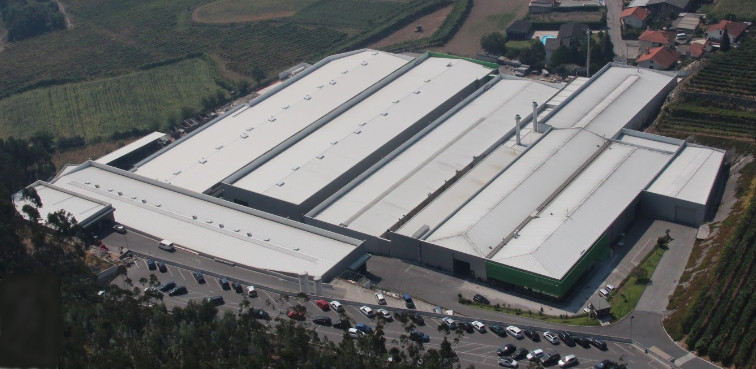
\includegraphics[scale=0.25]{./image/ROQ/ROQ_Pavilhoes.jpg}
\end{minipage}
\hfill
\begin{minipage}{0.45\linewidth}
\begin{itemize}
\item Industria de estamparia têxtil e embalagem\\
\item Produção, comercialização e assistência\\
\item 41 anos de atividade
\end{itemize}
\end{minipage}

\end{figure}

\end{frame}
%%%%%%%%%%%%%%%%%%%%%%%%%%%%%%%%%%%%%%%%%%%%%%%%%%%%%%%%%%%%%%%%%%%%%%%%%%%%%%%%%%%%%%%%%%%%%%%%%%%%%%%%%%%%%%%
\begin{frame}
\frametitle{1979-1983}
Sr. Manuel Sá se estabeleceu por conta própria, ocupando a garagem de uma habitação de um familiar, no Lugar de S.Roque (Freguesia de Riba de Ave, Concelho de Vila Nova de Famalicão), deu início a uma empresa vocacionada para a prestação de todo o tipo de serviços relativos à serralharia mecânica. Centrou desde logo a sua atividade nas empresas têxteis da região, onde a manutenção dos equipamentos, quase na sua totalidade importados, proporcionavam um mercado de trabalho com inúmeras oportunidades.
\end{frame}
%%%%%%%%%%%%%%%%%%%%%%%%%%%%%%%%%%%%%%%%%%%%%%%%%%%%%%%%%%%%%%%%%%%%%%%%%%%%%%%%%%%%%%%%%%%%%%%%%%%%%%%%%%%%%%%
\begin{frame}
\frametitle{1983-1984}
Entrada do Sr. Joaquim Sá é constituída uma sociedade por quotas, com capital social de 1 milhão de escudos e dois postos de trabalho, sendo atribuída a denominação de Serralharia Mecânica S.Roque, Lda.
\end{frame}
%%%%%%%%%%%%%%%%%%%%%%%%%%%%%%%%%%%%%%%%%%%%%%%%%%%%%%%%%%%%%%%%%%%%%%%%%%%%%%%%%%%%%%%%%%%%%%%%%%%%%%%%%%%%%%%
\begin{frame}
\frametitle{1984-2001}
A empresa criou a sua primeira máquina automática de estampar artigos têxteis com formato circular. Desde então dedicou-se à criação do fabrico destas máquinas, marcando definitivamente a evolução da empresa. Na mesma época também iniciou o fabrico de Estufas de Termofixação e de Rámulas. O seu crescimento levou ano após ano a um aumento progressivo do número de colaboradores, bem como à necessidade de a empresa procurar um espaço mais adequado à nova realidade.
\end{frame}
%%%%%%%%%%%%%%%%%%%%%%%%%%%%%%%%%%%%%%%%%%%%%%%%%%%%%%%%%%%%%%%%%%%%%%%%%%%%%%%%%%%%%%%%%%%%%%%%%%%%%%%%%%%%%%%
\begin{frame}
\frametitle{2001-2004}
Surge a divisão do laser, com a designação de "Roqlaser" cujo objectivo é o fabrico de peças metálicas, através da utilização de tecnologia de vanguarda na área do corte a laser, quinagem e soldadura.
\end{frame}
%%%%%%%%%%%%%%%%%%%%%%%%%%%%%%%%%%%%%%%%%%%%%%%%%%%%%%%%%%%%%%%%%%%%%%%%%%%%%%%%%%%%%%%%%%%%%%%%%%%%%%%%%%%%%%%
\begin{frame}
\frametitle{2004 até Hoje}
S.Roque tem vindo a ter uma evolução acentuada a nível financeiro, tecnológico e humano, para puder atuar num mercado cada vez mais competitivo. Investiu na construção de novos pavilhões, aquisição de novas máquinas e contratação de mão-de-obra profissional, de modo a puder continuar a acompanhar um mercado cada vez mais exigente.
\end{frame}
%%%%%%%%%%%%%%%%%%%%%%%%%%%%%%%%%%%%%%%%%%%%%%%%%%%%%%%%%%%%%%%%%%%%%%%%%%%%%%%%%%%%%%%%%%%%%%%%%%%%%%%%%%%%%%%
\begin{frame}
\frametitle{2015}
S.roque transformou-se em ROQ. Atendendo às necessidades do seculo XXI reconhecemos a necessidade de criar uma marca verdadeiramente global que consiga de uma forma eficaz transmitir mais de 30 anos de história, inovação, internacionalização e conhecimento.
\end{frame}
%%%%%%%%%%%%%%%%%%%%%%%%%%%%%%%%%%%%%%%%%%%%%%%%%%%%%%%%%%%%%%%%%%%%%%%%%%%%%%%%%%%%%%%%%%%%%%%%%%%%%%%%%%%%%%%
\begin{frame}
\frametitle{Produtos}
\begin{figure}[ht]
\begin{center}
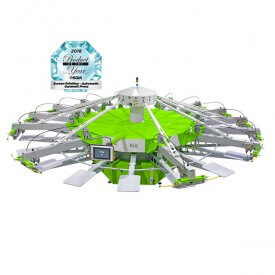
\includegraphics[scale=0.2]{"./image/ROQ/maquinas/ECO-P18_600x600-2-275x275.jpg"}
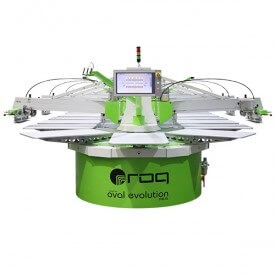
\includegraphics[scale=0.2]{"./image/ROQ/maquinas/EVO-600x600-275x275.jpg"}
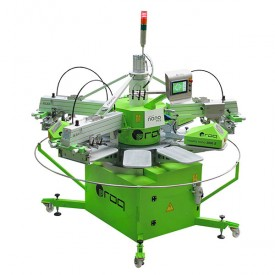
\includegraphics[scale=0.2]{"./image/ROQ/maquinas/nanop10-275x275.jpg"}
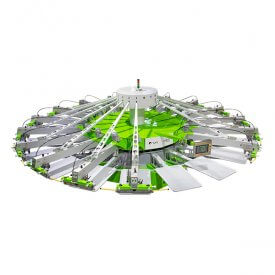
\includegraphics[scale=0.2]{"./image/ROQ/maquinas/NEXTP18-600x6001-275x275.jpg"}
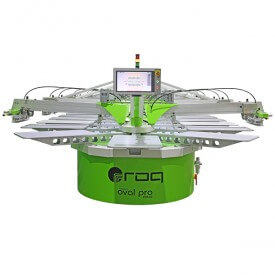
\includegraphics[scale=0.2]{"./image/ROQ/maquinas/PRO-600x600-275x275.jpg"}
\includegraphics[scale=0.2]{"./image/ROQ/maquinas/You-600x600-275x275"}
\end{center}
\begin{center}
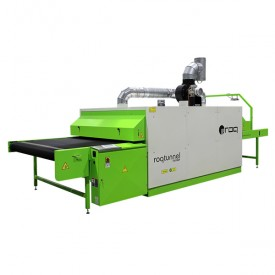
\includegraphics[scale=0.2]{"./image/ROQ/maquinas/T3018GP_600x600-275x275.jpg"}
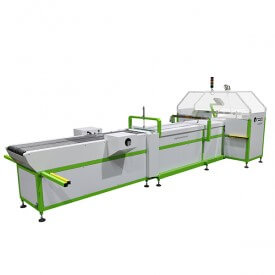
\includegraphics[scale=0.2]{"./image/ROQ/maquinas/600x6004-275x275.jpg"}
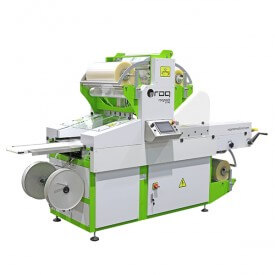
\includegraphics[scale=0.2]{"./image/ROQ/maquinas/600x6005-275x275.jpg"}
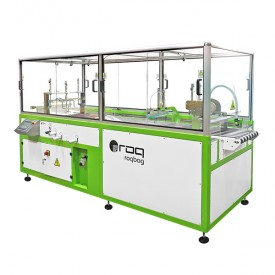
\includegraphics[scale=0.2]{"./image/ROQ/maquinas/600X600-275x275.jpg"}
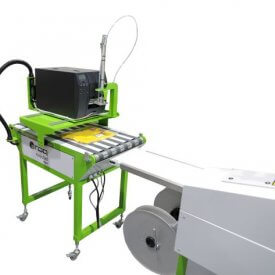
\includegraphics[scale=0.2]{"./image/ROQ/maquinas/DR7A6026_WEB1-275x275.jpg"}
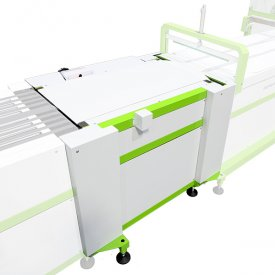
\includegraphics[scale=0.2]{"./image/ROQ/maquinas/ROQ-LABEL1-275x275.jpg"}
\end{center}
\end{figure}
\end{frame}
%%%%%%%%%%%%%%%%%%%%%%%%%%%%%%%%%%%%%%%%%%%%%%%%%%%%%%%%%%%%%%%%%%%%%%%%%%%%%%%%%%%%%%%%%%%%%%%%%%%%%%%%%%%%%%%
\section{Organização e sua Cultura}
%%%%%%%%%%%%%%%%%%%%%%%%%%%%%%%%%%%%%%%%%%%%%%%%%%%%%%%%%%%%%%%%%%%%%%%%%%%%%%%%%%%%%%%%%%%%%%%%%%%%%%%%%%%%%%%
\begin{frame}
\frametitle{Suas Características}
\begin{itemize}
\item Organização Privada com fins lucrativos
\item Hierarquia achatada
\item Departamento de supporte e produção
\item Desenvolvimento e montagem de maquinas
\item Prestadora de serviços
\item Implementação por produto
\item Divisão de trabalho
\item Ferramentas mais recentes \textbf{Solid Works}
\end{itemize}
\end{frame}
%%%%%%%%%%%%%%%%%%%%%%%%%%%%%%%%%%%%%%%%%%%%%%%%%%%%%%%%%%%%%%%%%%%%%%%%%%%%%%%%%%%%%%%%%%%%%%%%%%%%%%%%%%%%%%%
\begin{frame}
\frametitle{Sua Identidade}
\begin{block}{Missão}
A S.Roque tem como missão a constante inovação e criação de produtos de excelência na área da estamparia têxtil à peça. Para tal, aposta em múltiplos vetores complementares: tecnologia, qualidade e recursos humanos especializados. Estimula de forma persistente a sua veia empreendedora e internacional, promovendo para isso o contínuo aperfeiçoamento do seu serviço, em qualquer parte do mundo, mantendo-se fiel aos princípios éticos e de sustentabilidade.
\end{block}
\begin{alertblock}{Visão}
Trilhar um percurso sustentável de inovação, de expansão internacional, de excelência em todas as soluções que lançamos para o mercado, de qualidade absoluta, para nos mantermos como líder na nossa área de negócio
\end{alertblock}
\end{frame}
%%%%%%%%%%%%%%%%%%%%%%%%%%%%%%%%%%%%%%%%%%%%%%%%%%%%%%%%%%%%%%%%%%%%%%%%%%%%%%%%%%%%%%%%%%%%%%%%%%%%%%%%%%%%%%%
\begin{frame}
\frametitle{Sua Identidade}
\begin{exampleblock}{Valores}
\begin{itemize}
\setlength\itemsep{-0.3em}
\item Ação dentro dos princípios morais e éticos da empresa para com os seus stakeholders.
\item Atuação sempre no interesse dos nossos parceiros de forma a promover a sua satisfação e fidelização.
\item Excelência conseguida através de trabalho de equipa, competência e responsabilidade.
\item Qualidade absoluta.
\item Inovação promovida pelo ADN empreendedor da S. Roque.
\item Sustentabilidade ambiental e segurança.
\end{itemize}
\end{exampleblock}
\end{frame}
%%%%%%%%%%%%%%%%%%%%%%%%%%%%%%%%%%%%%%%%%%%%%%%%%%%%%%%%%%%%%%%%%%%%%%%%%%%%%%%%%%%%%%%%%%%%%%%%%%%%%%%%%%%%%%%
%%%%%%%%%%%%%%%%%%%%%%%%%%%%%%%%%%%%%%%%%%%%%%%%%%%%%%%%%%%%%%%%%%%%%%%%%%%%%%%%%%%%%%%%%%%%%%%%%%%%%%%%%%%%%%%
\section{Modelo Ogbonna \& Harris}
%%%%%%%%%%%%%%%%%%%%%%%%%%%%%%%%%%%%%%%%%%%%%%%%%%%%%%%%%%%%%%%%%%%%%%%%%%%%%%%%%%%%%%%%%%%%%%%%%%%%%%%%%%%%%%%
\begin{frame}
\frametitle{Estudo Ogbonna \& Harris}
\quad {\bf Estudo da relação entre as variáveis abaixo descritos:} \\
\vspace{.7cm}
\begin{minipage}[t]{.3\linewidth}
\quad Estilos de Liderança:
\begin{itemize}
\setlength\itemsep{-0.3em}
\item Participativo
\item Orientado as pessoas
\item Orientado as tarefas
\end{itemize}
\end{minipage}
\begin{minipage}[t]{.3\linewidth}
\quad Tipos de Cultura:
\begin{itemize}
\setlength\itemsep{-0.3em}
\item Inovadora
\item Competitiva
\item Burocrática
\item Comunitária
\end{itemize}
\end{minipage}
\begin{minipage}[t]{.3\linewidth}
\quad \textbf{Sucesso}:
\begin{itemize}
\setlength\itemsep{-0.3em}
\item Satisfação dos Clientes
\item Taxa crescimento vendas
\item Cotação no mercado
\item Vantagens Competitivas
\item Volume de vendas
\end{itemize}
\end{minipage}
\end{frame}
%%%%%%%%%%%%%%%%%%%%%%%%%%%%%%%%%%%%%%%%%%%%%%%%%%%%%%%%%%%%%%%%%%%%%%%%%%%%%%%%%%%%%%%%%%%%%%%%%%%%%%%%%%%%%%%
\begin{frame}
\frametitle{Modelo Ogbonna \& Harris}
Estudo feito a 322 Empresas na Inglaterra através de inquéritos deu este resultado:\\
\vspace{.2cm}
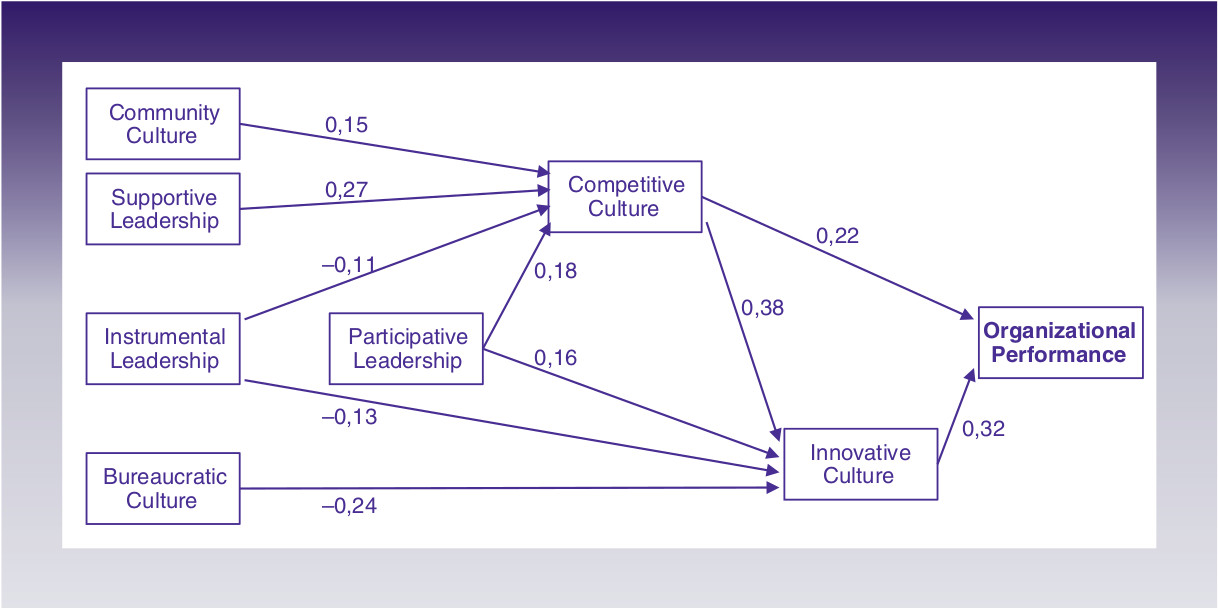
\includegraphics[scale=.25]{"./image/OB/Ogbonna & Harris.jpg"}
\end{frame}
%%%%%%%%%%%%%%%%%%%%%%%%%%%%%%%%%%%%%%%%%%%%%%%%%%%%%%%%%%%%%%%%%%%%%%%%%%%%%%%%%%%%%%%%%%%%%%%%%%%%%%%%%%%%%%%
\section{Cultura Organizacional}
%%%%%%%%%%%%%%%%%%%%%%%%%%%%%%%%%%%%%%%%%%%%%%%%%%%%%%%%%%%%%%%%%%%%%%%%%%%%%%%%%%%%%%%%%%%%%%%%%%%%%%%%%%%%%%%
\begin{frame}
\frametitle{\textcolor{green}{ROQ}}
\tiny
\begin{table}[h!]
\begin{adjustbox}{max width=\textwidth}
\begin{tabular}{ |c|l|c| }
\hline
\rowcolor[gray]{0.5}
Nº & Inquérito para Determinar a Cultura Organizacional & \makecell[l]{Resp \\ 1 \; - \; 7} \\
\hline
\cellcolor{brown} 1. & \makecell[l]{A organização preocupa-se com o crescimento e a aquisição de novos recursos, \\ e procura responder a novos desafios.} & \\
\hline
\cellcolor{brown} 2. & \makecell[l]{A organização é dinâmica e empreendedora. \\ As pessoas estão dispostas a correr riscos.} & \\
\hline
\cellcolor{brown} 3. & \makecell[l]{Existe um elevado empenho na inovação e no desenvolvimento. \\ Procuramos ser os primeiros.} & \\
\hline
\cellcolor{brown} 4. & \makecell[l]{Consideram-se os melhores gestores os que são empreendedores, \\ Inovadores e tomadores de riscos.} & \\
\hline
\cellcolor{red} 5. & Existe uma elevada ênfase nas tarefas e no alcance de objetivos. & \\
\hline
\cellcolor{red} 6. & Considera-se que os melhores gestores são produtores e técnicos. & \\
\hline
\cellcolor{red} 7. & \makecell[l]{A organização valoriza as ações competitivas, \\ o sucesso e o alcance de objetivos mensuráveis.} & \\
\hline
\cellcolor{red} 8. & \makecell[l]{A organização é orientada para a produção. \\ Uma das maiores preocupações é fazer o que tem que ser feito. \\ Os empregados não estão muito envolvidos do ponto de vista pessoal.} & \\
\hline
\cellcolor{orange} 9. & A organização valoriza muito as regras e as políticas formais. & \\
\hline
\cellcolor{orange} 10. & \makecell[l]{A organização é muito formalizada e estruturada. \\ Os procedimentos estabelecidos orientam o que as pessoas devem fazer.} & \\
\hline
\cellcolor{orange} 11. & Os melhores gestores são considerados os que são coordenadores ou organizadores. & \\
\hline
\cellcolor{orange} 12. & Na organização valoriza-se a permanência, a estabilidade e a eficiência. & \\
\hline
\cellcolor{yellow} 13. & Valoriza-se muito a lealdade, a tradição e o empenhamento na organização. & \\
\hline
\cellcolor{yellow} 14. & A organização é uma espécie de grande família. & \\
\hline
\cellcolor{yellow} 15. & Valoriza-se muito a coesão e os recursos humanos. & \\
\hline
\cellcolor{yellow} 16. & \makecell[l]{Considera-se que os melhores gestores são os que atuam como mentores, \\ sábios ou figuras paternais/maternais.} & \\
\hline
\end{tabular}
\end{adjustbox}
\end{table}
\end{frame}
%%%%%%%%%%%%%%%%%%%%%%%%%%%%%%%%%%%%%%%%%%%%%%%%%%%%%%%%%%%%%%%%%%%%%%%%%%%%%%%%%%%%%%%%%%%%%%%%%%%%%%%%%%%%%%%
\begin{frame}
\begin{table}[h!]
{\small
\begin{tabular}{|l|c|c|}
\hline
                                                                                                    & Média do Inquerito & \begin{tabular}[c]{@{}l@{}}Ogbonna \& Harris\\ (2000)\end{tabular} \\ \hline
\cellcolor[HTML]{C0C0C0}\begin{tabular}[c]{@{}l@{}}Cultura de inovação\\ {[}1-4{]}\end{tabular}     & 5,4 & 4,6 \cellcolor[HTML]{EFEFEF}                                           \\ \hline
\cellcolor[HTML]{C0C0C0}\begin{tabular}[c]{@{}l@{}}Cultura de Competição\\ {[}5-8{]}\end{tabular}   & 5,3 & 4,2 \cellcolor[HTML]{EFEFEF}                                           \\ \hline
\cellcolor[HTML]{C0C0C0}\begin{tabular}[c]{@{}l@{}}Cultura Burocrática\\ {[}9-12{]}\end{tabular}    & 4,7  & 4,3 \cellcolor[HTML]{EFEFEF}                                           \\ \hline
\cellcolor[HTML]{C0C0C0}\begin{tabular}[c]{@{}l@{}}Cultura de Comunidade\\ {[}13-16{]}\end{tabular} & 5  & 4,6 \cellcolor[HTML]{EFEFEF}                                           \\ \hline
\end{tabular}
}
\end{table}
\end{frame}
%%%%%%%%%%%%%%%%%%%%%%%%%%%%%%%%%%%%%%%%%%%%%%%%%%%%%%%%%%%%%%%%%%%%%%%%%%%%%%%%%%%%%%%%%%%%%%%%%%%%%%%%%%%%%%%
\section{Conclusões}
%%%%%%%%%%%%%%%%%%%%%%%%%%%%%%%%%%%%%%%%%%%%%%%%%%%%%%%%%%%%%%%%%%%%%%%%%%%%%%%%%%%%%%%%%%%%%%%%%%%%%%%%%%%%%%%
\begin{frame}
\frametitle{\textcolor{green}{ROQ}}
Pelo resultado do inquérito feito pode-se dizer que a S.Roque aponta para uma cultura predominantemente \textcolor{blue}{inovadora}, com um grau elevado de incerteza devido ter muito poucas amostras. Com este inquérito, deu para perceber que cada individuo tem uma perceção diferente da organização, o que leva a crer que a S.Roque não tem uma cultura forte. O estilo de liderança é mais orientado ás tarefas, ou seja, uma liderança transacional ou instrumental.
\end{frame}
%%%%%%%%%%%%%%%%%%%%%%%%%%%%%%%%%%%%%%%%%%%%%%%%%%%%%%%%%%%%%%%%%%%%%%%%%%%%%%%%%%%%%%%%%%%%%%%%%%%%%%%%%%%%%%%
\begin{frame}
\frametitle{\textcolor{green}{ROQ}}
A S.Roque tem orgulho em afirmar que é o primeiro no nosso mercado interno e destaca-se internacionalmente. O seu sucesso poderá ser medido recorrendo ao \textcolor{blue}{benchmarking} que o confirma. Ao nível de satisfação dos seus clientes o \textcolor{blue}{scorecard management} não foi possível obter nenhuma informação, e seu site não tem indicações de tal. O \textcolor{blue}{Banco de Portugal} também é outra fonte onde é possível verificar o sucesso da organização quanto ao histórico do seu capital. O desempenho da organização pode no fim ser demonstrado através da sua eficácia e eficiência.\\
\end{frame}
%%%%%%%%%%%%%%%%%%%%%%%%%%%%%%%%%%%%%%%%%%%%%%%%%%%%%%%%%%%%%%%%%%%%%%%%%%%%%%%%%%%%%%%%%%%%%%%%%%%%%%%%%%%%%%%
\begin{frame}
\centering
\Huge \textcolor{blue}{\textbf{FIM}}
\end{frame}
%%%%%%%%%%%%%%%%%%%%%%%%%%%%%%%%%%%%%%%%%%%%%%%%%%%%%%%%%%%%%%%%%%%%%%%%%%%%%%%%%%%%%%%%%%%%%%%%%%%%%%%%%%%%%%%
%%%%%%%%%%%%%%%%%%%%%%%%%%%%%%%%%%%%%%%%%%%%%%%%%%%%%%%%%%%%%%%%%%%%%%%%%%%%%%%%%%%%%%%%%%%%%%%%%%%%%%%%%%%%%%%
\end{document}
%%%%%%%%%%%%%%%%%%%%%%%%%%%%%%%%%%%%%%%%%%%%%%%%%%%%%%%%%%%%%%%%%%%%%%%%%%%%%%%%%%%%%%%%%%%%%%%%%%%%%%%%%%%%%%%